\chapter{Bases de Docker}
\label{ch:docker}

\section{Introduction}
Dans ce chapitre nous allons parler du fonctionnement de \emph{Docker} et \emph{Docker COmpose}. Ce chapitre est réalisé sous le ton d'un cours d'introduction à Docker, afin de pouvoir transmettre les connaissance de base a l'utilisation et à la modification du travail réalisé lors de cette thèse. Cela passera entre autre par certain exemple et code qui seront fournit en annexe notamment.

Docker permet l'execution de code dans un conteneurs indépendant de vote systeme hôte. 

\subsection{Utilisations}
\subsection{Compatibilité inter-OS}
Docker permet d'éviter les problemes liés aux différences entre les environnements d'execution. En effet, lorsque l'on execute un code avec Docker ont contrôle exactement l'états et le type d'environnement d'execution. Cela rend donc possible l'execution d'un code sous différent \gls{os} hôte (OSX, Linux, Windows).

Mais pourquoi ne pas utiliser une simple machine virtuelle ? Une première différence entre une machine virtuelle et DOcker est le fait que Docker n'encapsule pas tout un \gls{os}, ceci permet une execution beaucoup plus rapide, et c'est bien se que l'on cherche dans ce travail.

\begin{figure}[H] 
\centering 
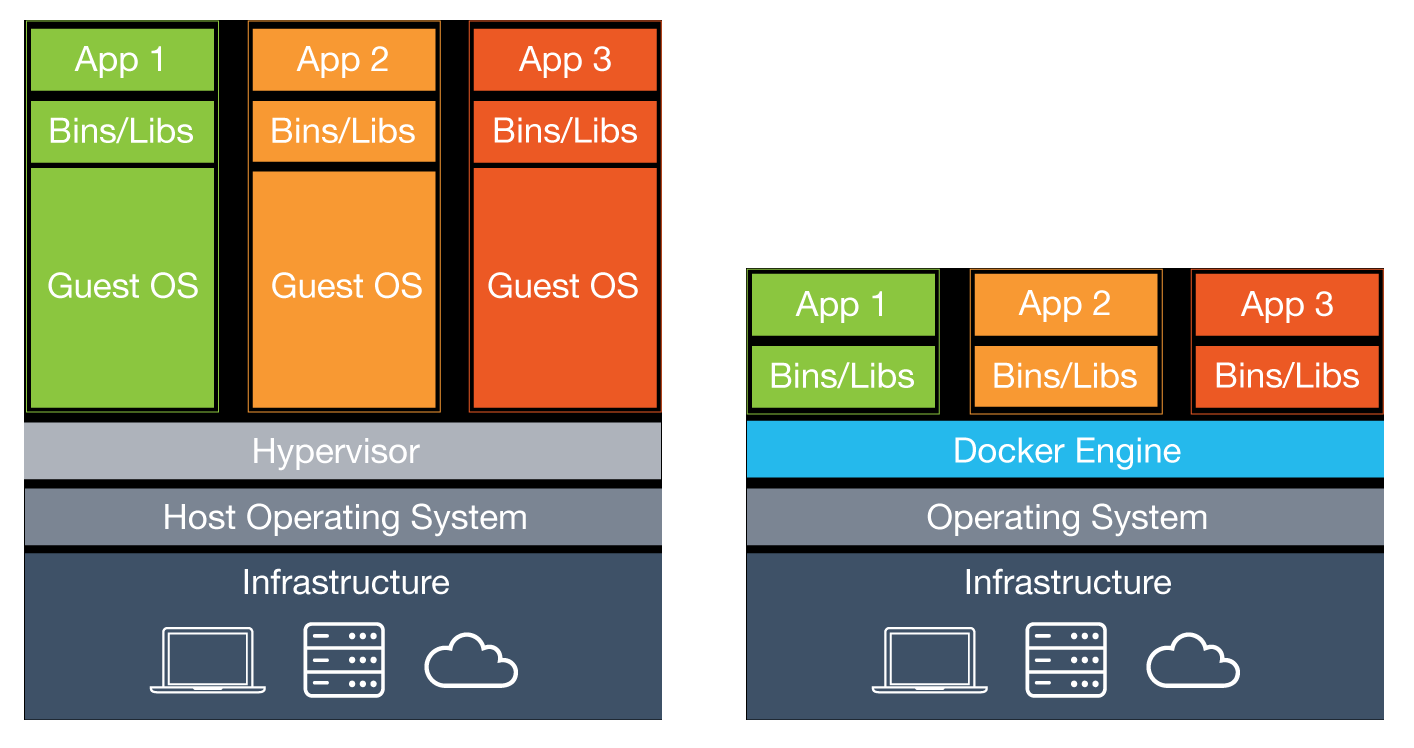
\includegraphics[width=1\columnwidth]{img/vm-vs-docker-container} 
\caption[vm vs Docker]{Virtual machine vs Docker}
\label{fig:vs} 
\end{figure}

\subsection{Miracle or illusion}
Je tiens ici à faire une mise en garde vis-à-vis de l'utilisation de Docker. Dans sont utilisation Docker est, à mon sens, une solution assez miraculeuse, notamment par le fait que l'on peu partage une application sans se poser de question sur l'hôte cible. Mais attention Docker n'est pas aussi miraculeux que cela dans le développement d'une solution applicative. En effet, il peu parfois etres compliquer d'arriver du premier coup à réaliser se que l'on souhaite.

Docker n'est donc pas une solution miracle, mais présente beaucoup d'avantages en terme d'execution standardisé, de partage de code et de déploiment.

\section{Pré-requis}
\subsection{Connaissance}
Il est necessaire d'etres à laise avec l'\gls{os} Linux et l'utilisation de commande UNIX. En effet, la pluspart du temps les conteneurs utiliserons un systeme Linux. Pour plus d'information cf. ci-après.


\subsection{Installations}
\lstset{language=bash}
\lstset{
    frame=single,
    breaklines=true,
    postbreak=\raisebox{0ex}[0ex][0ex]{\ensuremath{\color{red}\hookrightarrow\space}}
}

\subsubsection{Installation Docker}
\begin{lstlisting}[frame=single]
$ sudo apt-get update
$ sudo apt-get install apt-transport-https ca-certificates
$ sudo apt-key adv --keyserver hkp://p80.pool.sks-keyservers.net:80 --recv-keys 58118E89F3A912897C070ADBF76221572C52609D

$ sudo apt-add-repository 'deb https://apt.dockerproject.org/repo ubuntu-xenial main'
$ sudo apt-get update
$ sudo apt-cache policy docker-engine
$ sudo apt-get install -y docker-engine
$ sudo systemctl status docker
\end{lstlisting}

Vous devriez maintenant voir une sortie console semblable a celle de la figure \ref{fig:dockerservices}:

\begin{figure}[H] 
\centering 
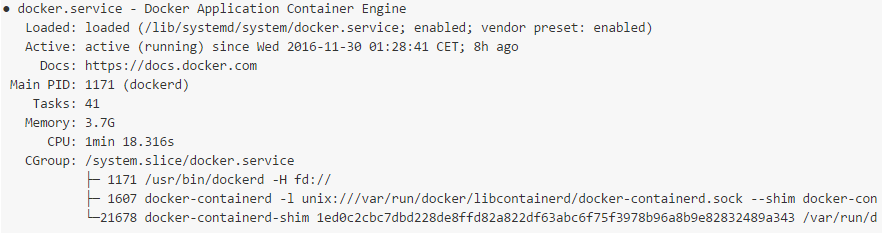
\includegraphics[width=1\columnwidth]{img/docker-services} 
\caption[docker services]{Services Docker opperationnel}
\label{fig:dockerservices} 
\end{figure}

Il faut à présent configurer Docker pour votre utilisateur hôte.

\begin{lstlisting}[frame=single]
$ sudo usermod -aG docker $(whoami)
\end{lstlisting}

A se point ci, il vous faut redémarer votre machine.

\subsubsection{Installation Docker-compose (1.9)}

\begin{lstlisting}[frame=single]
$ curl -L "https://github.com/docker/compose/releases/download/1.9.0/docker-compose-$(uname -s)-$(uname -m)" -o /usr/local/bin/docker-compose
$ sudo chmod +x /usr/local/bin/docker-compose
$ docker-compose --version
\end{lstlisting}

Vous devriez à présent obtenir la sortie console suivante:
\begin{lstlisting}[frame=single]
docker-compose version: 1.9.0
\end{lstlisting}

\subsection{Téléchargements}

\section{Fonctionnement}
\subsection{Docker}
Il faut commencer par clarifier de quoi ont parle lorsque l'on utilise le mot conteneur. Il s'agit d'une \emph{enveloppe} virtuelle permettant de packager une application ou un code avec toutes les dépendance necessaire au fonctionnement de l'application. On package donc les fichiers source, librairies, runtime, outils, fichiers, base de données, etc. 

Un conteneur n'embarque pas de \gls{os}, il s'appuie sur celui de l'hôte sur lequel il est deployé. Ce qui rend un conteneurs baucoup plus légé qu'une machine virtuelle \ref{fig:vs}.

Il faut également spécifier que Docker opère une isolation, des conteneurs, au niveau du système d'explotation. 

Un conteneurs DOcker est decrit à l'aide d'un simple fichier \emph{.Dockerfile}, il décrit la création du conteneur, en détails. On peut personnaliser cette description de manière très détaillée. 

Il faut voir une application réalisé avec Docker comme une somme de micro-services. Nous verrons dans la section suivante des exemples basiques d'application DOcker. Le but étant de:

\begin{itemize}
\item rendre l'application d'avantage élastique;
\item Améliorer les performance;
\item Le déploiement continue est facilité. On peu relancer les services independament les un des autres.
\end{itemize}


\subsection{Docker-compose}
Docker-compose permet de définir et d'executer des application multi-conteneurs. En effet, sans compose il fallait lancer les différent services de votre application soit manuellement soit en utilisant des scripts.

Compose utilise un fichier de composition, \emph{docker-compose.yml}, afin de configurer une application Docker. Ce qui permet de lancer une application à l'aide d'une seule commande. 

Pour résumer, une application Docker, utilisant Compose, est la combinaison de trois étapes:

\begin{enumerate}
\item Définir les différent Dockerfile des vos micro-services composant l'application;
\item Définir les services qui seront utilisé dans le compose, leurs relation et leurs configurations;
\item Lancer l'application avec la simple commande, \emph{docker-compose up}.
\end{enumerate}


\section{Exemples}
\subsection{simple pull, build et run}
\subsection{Serveur Web}
\subsection{Biopython}
\subsection{Parallélisation}

\section{Conclusion}
\subsection{Docker}
\subsection{Alternatives}
































